As mentioned above, \acrshort{idpcndu}, which has also been proven to be NP-complete~\cite{maggi2018domain}, is a variant of the original \gls{idpcdu}. In general, previous approaches for \gls{idpcdu} or \acrshort{idpcndu} are often unable, or they have to go through several transformation steps to solve the remaining one. Our proposed algorithm, on the other hand, can be applied to both problems. 

Since \acrshort{idpcndu} no longer assigns domains on edges, there is only one edge with the smallest weight between any two nodes~\cite{binh2021two} (See Figure~\ref{fig:idpc-ndu-example}). Then, Equation~\ref{equation:edge_pick} is changed to Equation~\ref{equation:edge_pick_ndu} as follows.
\begin{equation}
	\label{equation:edge_pick_ndu}
	p_e(t) = 
	\frac{[\tau_e(t)]^{\alpha} \cdot [\eta_e(t)]^{\beta} \cdot  [P_n(t)]^{\gamma}}{\Sigma_{h \in Adj(v_i)} [\tau_h(t)]^{\alpha} \cdot [\eta_h(t)]^{\beta} \cdot [P_h(t)]^{\gamma}},
\end{equation}
where $P_n$ is the domain's priority of the node to which edge $e$ leads. $Adj(v_i)$ now includes all nodes that ant $k$ has not yet traversed, whose domains satisfy the \gls{du} and $Domain~Blacklist~Check$, and the edges directing to these nodes fulfill the $Checksum$.
Also, for the $Domain~Blacklist~Check$ component, each node now still contains a blacklist. However, it will store the stuck domain sequence of the nodes that ants have visited.
\bigskip
\setlength{\intextsep}{3pt}
\renewcommand{\scalefigure}{.9}
\begin{figure}[htbp]
	\centering
	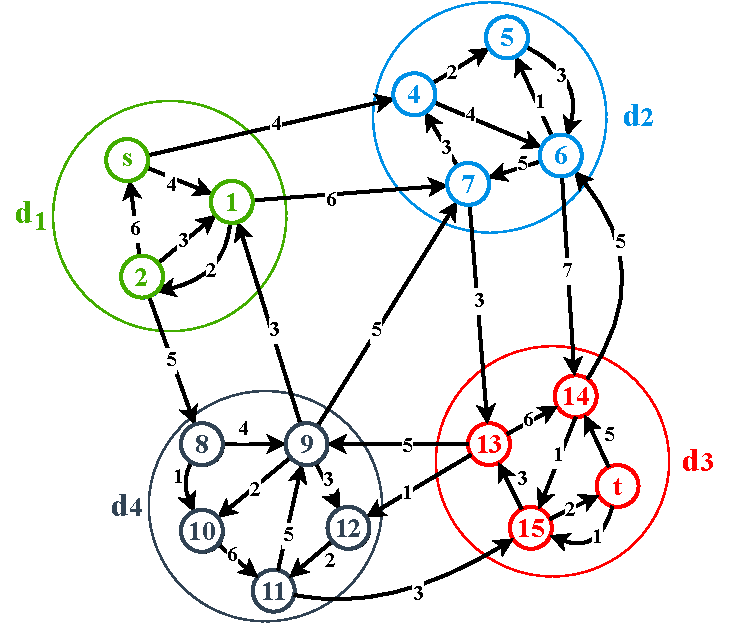
\includegraphics[scale=\scalefigure]{Figures/chap 3/IDPC-NDU.pdf}
	\caption{An example input graph of the \gls{idpcndu}}
	\label{fig:idpc-ndu-example}
\end{figure}